%% bare_jrnl_compsoc.tex
%% V1.4a
%% 2014/09/17
%% by Michael Shell
%% See:
%% http://www.michaelshell.org/
%% for current contact information.
%%
%% This is a skeleton file demonstrating the use of IEEEtran.cls
%% (requires IEEEtran.cls version 1.8a or later) with an IEEE
%% Computer Society journal paper.
%%
%% Support sites:
%% http://www.michaelshell.org/tex/ieeetran/
%% http://www.ctan.org/tex-archive/macros/latex/contrib/IEEEtran/
%% and
%% http://www.ieee.org/

%%*************************************************************************
%% Legal Notice:
%% This code is offered as-is without any warranty either expressed or
%% implied; without even the implied warranty of MERCHANTABILITY or
%% FITNESS FOR A PARTICULAR PURPOSE! 
%% User assumes all risk.
%% In no event shall IEEE or any contributor to this code be liable for
%% any damages or losses, including, but not limited to, incidental,
%% consequential, or any other damages, resulting from the use or misuse
%% of any information contained here.
%%
%% All comments are the opinions of their respective authors and are not
%% necessarily endorsed by the IEEE.
%%
%% This work is distributed under the LaTeX Project Public License (LPPL)
%% ( http://www.latex-project.org/ ) version 1.3, and may be freely used,
%% distributed and modified. A copy of the LPPL, version 1.3, is included
%% in the base LaTeX documentation of all distributions of LaTeX released
%% 2003/12/01 or later.
%% Retain all contribution notices and credits.
%% ** Modified files should be clearly indicated as such, including  **
%% ** renaming them and changing author support contact information. **
%%
%% File list of work: IEEEtran.cls, IEEEtran_HOWTO.pdf, bare_adv.tex,
%%                    bare_conf.tex, bare_jrnl.tex, bare_conf_compsoc.tex,
%%                    bare_jrnl_compsoc.tex, bare_jrnl_transmag.tex
%%*************************************************************************

% *** Authors should verify (and, if needed, correct) their LaTeX system  ***
% *** with the testflow diagnostic prior to trusting their LaTeX platform ***
% *** with production work. IEEE's font choices and paper sizes can       ***
% *** trigger bugs that do not appear when using other class files.       ***                          ***
% The testflow support page is at:
% http://www.michaelshell.org/tex/testflow/

\documentclass[10pt,conference,onecolumn,compsoc]{IEEEtran}

\usepackage{hyperref}
\usepackage{enumitem}
\setlist[itemize]{leftmargin=3 cm}
\setlist[enumerate]{leftmargin=3cm}

% *** CITATION PACKAGES ***
%
\ifCLASSOPTIONcompsoc
  % IEEE Computer Society needs nocompress option
  % requires cite.sty v4.0 or later (November 2003)
  \usepackage[nocompress]{cite}
\else
  % normal IEEE
  \usepackage{cite}
\fi
% cite.sty was written by Donald Arseneau
% V1.6 and later of IEEEtran pre-defines the format of the cite.sty package
% \cite{} output to follow that of IEEE. Loading the cite package will
% result in citation numbers being automatically sorted and properly
% "compressed/ranged". e.g., [1], [9], [2], [7], [5], [6] without using
% cite.sty will become [1], [2], [5]--[7], [9] using cite.sty. cite.sty's
% \cite will automatically add leading space, if needed. Use cite.sty's
% noadjust option (cite.sty V3.8 and later) if you want to turn this off
% such as if a citation ever needs to be enclosed in parenthesis.
% cite.sty is already installed on most LaTeX systems. Be sure and use
% version 5.0 (2009-03-20) and later if using hyperref.sty.
% The latest version can be obtained at:
% http://www.ctan.org/tex-archive/macros/latex/contrib/cite/
% The documentation is contained in the cite.sty file itself.

% *** GRAPHICS RELATED PACKAGES ***
%
\ifCLASSINFOpdf
   \usepackage[pdftex]{graphicx}
 
\else
 
\fi
% graphicx was written by David Carlisle and Sebastian Rahtz. It is
% required if you want graphics, photos, etc. graphicx.sty is already
% installed on most LaTeX systems. The latest version and documentation
% can be obtained at: 
% http://www.ctan.org/tex-archive/macros/latex/required/graphics/
% Another good source of documentation is "Using Imported Graphics in
% LaTeX2e" by Keith Reckdahl which can be found at:
% http://www.ctan.org/tex-archive/info/epslatex/
%
% latex, and pdflatex in dvi mode, support graphics in encapsulated
% postscript (.eps) format. pdflatex in pdf mode supports graphics
% in .pdf, .jpeg, .png and .mps (metapost) formats. Users should ensure
% that all non-photo figures use a vector format (.eps, .pdf, .mps) and
% not a bitmapped formats (.jpeg, .png). IEEE frowns on bitmapped formats
% which can result in "jaggedy"/blurry rendering of lines and letters as
% well as large increases in file sizes.
%
% You can find documentation about the pdfTeX application at:
% http://www.tug.org/applications/pdftex

% *** PDF, URL AND HYPERLINK PACKAGES ***
%
\usepackage{url}
% url.sty was written by Donald Arseneau. It provides better support for
% handling and breaking URLs. url.sty is already installed on most LaTeX
% systems. The latest version and documentation can be obtained at:
% http://www.ctan.org/tex-archive/macros/latex/contrib/url/
% Basically, \url{my_url_here}.



\begin{document}

% TITLE ************************************************************************* %

% Title
\begin{figure}
\centering
{\Huge CYBERNUKE}\\
POST-APOCALYPTIC CYBERPUNK ROGUELITE\\
J. Kenneth Wallace, Vance Brender-A-Brandis\\
\end{figure}
% Abstract
\IEEEtitleabstractindextext{
\begin{abstract}
CYBERNUKE is a roguelite game developed in the C\# WPF framework. You play as an amnesiac cyborg who awakens in the middle of a destroyed futuristic city and must recover their memories. The game combines a post-apocalyptic and cyberpunk setting to create a unique atmosphere not previously explored by other games. The setting of the game is inspired by popular stories such as \emph{Fallout}, \emph{Cyberpunk 2077}, and other game series like \emph{Dark Souls} and \emph{Megami Tensei}.
\end{abstract}
}
\IEEEdisplaynontitleabstractindextext
\IEEEpeerreviewmaketitle



% INTRODUCTION ************************************************************************* %
\section{Introduction}

For this project we aim to create a video game to gain experience with C\#, WPF, and game design. We called the game CYBERNUKE, combining the game's cyberpunk and post-apocalyptic elements into a single title.

The setting of the game is rooted in the cyberpunk genre, taking place in a massive futuristic city where buildings as tall as the Empire State Building are commonplace, gangs are armed with high-tech laser guns, and the wealth gap is at its widest. On a peaceful day in the twenty-first century, the city is attacked by an unknown power, which is followed by a nuclear explosion and the displacement of the entire city into another dimension. The story's cyberpunk portion is inspired by the game \emph{Cyberpunk 2077}, while the post-apocalyptic portion is inspired by \emph{Fallout} and other post-apocalyptic games. 

CYBERNUKE's gameplay is influenced by games such as the \emph{Shin Megami} and \emph{Dark Souls} series. Shin Megami inspired the game's turn-based combat, while Dark Souls inspired the overworld map and exploration. Moreover, CYBERNUKE is heavily influenced by the roguelike genre, particularly games like \emph{Slay the Spire}, \emph{The Binding of Isaac}, and \emph{FTL: Faster Than Light}.

We hope that those who enjoy the gameplay and story of the works that inspired CYBERNUKE will enjoy the game we make as well.

\subsection{Audience}
CYBERNUKE has a diverse setting, story, and gameplay that draws inspiration from a wide range of games and stories. We want to draw in fans by fusing two sizable genres—cyberpunk and post-apocalyptic—and putting it into a roguelite game. Those looking for gameplay should expect turn-based combat and a top-down world filled with exploration and encounters akin to \emph{Pokémon}. Those who come for the story will be treated to a mysterious tale about someone piecing together their memories in a new, hostile cyberpunk hell. 

%Cosmetic Page Break
\pagebreak
\subsection{Background}
CYBERNUKE is inspired by roguelike games, but it does not completely follow them, making CYBERNUKE a rogue-\emph{lite}. Roguelite games are a subgenre of roguelike games. The Berlin Interpretation of a “roguelike,” developed at the 2008 International Roguelike Development Conference, is the most widely accepted definition. It specifies that all roguelikes must have the following characteristics\cite{IEEEhowto:roguelite_2}:
\begin{enumerate}
\item Permadeath: the player has one life per game.
\item Random environment generation: no map or encounter is ever the same.
\item Exploration and discovery: the player explores the map and finds items.
\item Turn-based, grid-based, non-modal gameplay: all actions are turn-based, on a grid map, on a single screen that holds all windows and doesn't change.
\item Hack-n-slash: the player defeats a lot of monsters.
\item Resource management: the player manages a limited amount of resources.
\end{enumerate}
Permadeath, random environment generation, and non-modal gameplay are not included in CYBERNUKE. As such, our game is classified as a roguelite because it lacks most of the required features. Specifically, roguelite as used by CYBERNUKE means the player has infinite lives, explores a pre-built map with loot spread out, encounters enemies at fixed rates, fights in turn-based combat, and manages a limited amount of resources.

CYBERNUKE's setting is a hybrid of two genres: cyberpunk and post-apocalyptic.
Cyberpunk is defined as a \emph{"science-fiction subgenre characterized by countercultural antiheroes trapped in a dehumanized, high-tech future,"}\cite{IEEEhowto:cyberpunk} or a dystopian future full of holograms, lasers, and crime. The post-apocalyptic genre is defined by the collapse of society as a result of a disaster, with a few survivors forming small civilizations. The combination of these two genres serves as the foundation for the rest of the story and gameplay. 

\subsection{Impacts}
If enough effort is put in, CYBERNUKE has the potential to amass a sizable fan base. An optimistic estimate would be that CYBERNUKE reaches a large audience that plays, discusses, and enjoys the game in general. The game would then inspire others to create stories or games in the same hybrid cyberpunk-post-apocalyptic genre. A more realistic estimate would be that the game is simply released and is only played by a small number of people. Expecting too much from such a small game is unrealistic. 

\subsection{Challenges}
Three big challenges will need to be overcome in this project:
\begin{enumerate}
\item Inexperience in C\# and WPF
\item Clear communication of ideas and implementations
\item Beating the time limit
\item How to design a game
\end{enumerate}
We've both never worked with the WPF framework, let alone C\#. As the project progresses, we will have to learn how to work with both. This can be mitigated by reading documentation or watching tutorials.

Clear communication can also be a big issue and can stop work if people aren't on the same page. What makes this worse is that we are both inspired by different games which makes it difficult to communicate ideas of one game that the other person hasn't experienced. The clear solution to a lack of clear communication is using standardized methods of communication like UMLs and Diagrams. UML and Discord will definitely be the work-horses of communication throughout the project.

Another issue is the project's time frame. Having to not only learn but also implement a large number of designs in a short period of time will be stressful, but it should be possible.

The most serious issue is that we have no experience designing games. There is a significant difference between playing and creating a game, which will need to be addressed as we continue to work. 

%Tactical Page Break
\pagebreak
% SCOPE ******************************************************************************** %
\section{Scope}
In order of importance, these are the fundamental game mechanics that must be implemented for \emph{CYBERNUKE} to be considered functional:
\begin{flushleft}
1. Operational Interfaces:
The Operational Interfaces are the menus that the player uses to interact with the game. (Main Menu, Combat Menu, Town Menu, Overworld Menu, Cutscene Menu).

2. Menu Switching: The ability to switch between Menus.

3. Secondary Interfaces: The Secondary Interfaces are other menus that are accessed within other menus (Pause Menu).

4. Enemies: Enemies and Enemy party files to load in enemies and groups of those enemies from.

5. Overworld Maps: The ability to create Overworld maps and render them onto the screen from a file.

6. Character-Map Interaction: The ability to move a player's character while they are on the map and the ability to interact with parts of that map as the player.

7. Enemy Encounters: Enemies are the monsters/humans that the player will encounter throughout the game. Enemy Encounters refers to how you will find monsters in the first place, which is primarily done through a "percent encounter" system akin to the old \textit{Pokemon} games.

8. Combat: Combat refers to fights between the player character and enemies in this game, which will be turn-based. Combat happens inside the Combat Menu.

9. Companions and Party System: Multiple player characters (up to 4) to bring into combat.

10. Basic Item System: A bare-bones item equip system that lets players equip different armor and weapons.
\end{flushleft}


After the fundamental game mechanics are in place, additional features that flesh out the game can be added.

Possible stretch-goal features:
\begin{flushleft}
1. Items, Loot, Weapons, Armor: A fully fleshed out equipment and item system.

2. Currency and Merchants: A money system with merchants you can find in Towns and buy items from.

3. Leveling System: Leveling system for players and enemies that scale in difficulty the higher the level you are.

4. More Enemy Types: Different types of unique enemies.

5. Saving and Loading: The ability to save and load the game, with an autosave for when you need to quit in the overworld and a proper save-load in the towns.

6. Hacking Puzzles: In-game puzzles that allow you to access certain areas of the map.

7. Story Content: A story tied to the game.
\end{flushleft}



\subsection{Requirements}
The required mechanics for the game to function at a basic level are defined in the first part of the scope. These mechanics are required as they are the foundation of the game's most basic actions such as traversing menus, moving around the map, viewing your character's stats, and fighting enemies.

The non-required mechanics for the game are defined in the second part of the scope. These are taken from other finished roguelite games and are not required for the game to function but for fleshing the game out into a more appealing state for the audience. They build upon the foundation laid by the functional mechanics to create something more than a roguelite mockup.

\subsubsection{Functional}
\begin{itemize}
\item User must be able to navigate the main menu.
\item User must be able to interact with the overworld menu.
\item User must be able to examine the stats of their character(s).
\item User must be able to interact with the combat menu.
\item User must be able to interact with the town menu.
\end{itemize}

\subsubsection{Non-Functional}
\begin{itemize}
\item User must be able to manage their inventory (Equip armor \& weapons, use items).
\item User must be able to shop with merchants in towns.
\item User must be able to upgrade their base stats when leveling up.
\item User must be able to save and load in the town menu.
\item Game must be able to autosave when leaving while user is in overworld menu.
\end{itemize}

\subsection{Use Cases}
\begin{table}
\centering
\begin{tabular}{|c|c|c|c|c|}
\hline
Use Case ID & Use Case Name & Primary Actor & Complexity & Priority \\
\hline \hline
1 & Main Menu: Start Demo & Player & Low & 1\\
\hline
2 & Main Menu: Change Options & Player & Med & 1\\
\hline
3 & Main Menu: Exit Game & Player & Low & 1\\
\hline
4 & Overworld Menu: Move Player & Player & Med & 1\\
\hline
5 & Overworld Menu: Toggle Pause Menu & Player & Low & 1\\
\hline
6 & Overworld Menu: Toggle Map & Player & Low & 1\\
\hline
7 & Overworld Menu: Interact & Player & Med & 1\\
\hline
8 & Pause Menu: Equip Item & Player & Med & 3\\
\hline
9 & Pause Menu: View Map & Player & Low & 3\\
\hline
10 & Pause Menu: Close Menu & Player & Low & 1\\
\hline
11 & Pause Menu: Exit Game & Player & Low & 1\\
\hline
12 & Combat Menu: Attack Enemy & Player & Med & 1\\
\hline
13 & Combat Menu: Wait & Player & Low & 1\\
\hline
14 & Combat Menu: Flee & Player & Low & 1\\
\hline
15 & Town Menu: Interact with NPC & Player & Low & 1\\
\hline
16 & Town Menu: Exit Town & Player & Low & 1\\
\hline

\end{tabular}
\caption{Cybernuke use case table}
\label{tab:useCaseIndex}
\end{table}


\begin{itemize}
\item[Use Case Number:] 1
\item[Use Case Name:] Start Demo
\item[Description:] Player is in the main menu and wants to start the demo.
\end{itemize}
\begin{enumerate}
\item Player is in the main menu.
\item Player clicks on “Start Demo”.
\item The main menu is closed and the overworld menu is opened.
\item[Termination Outcome:] The demo is started for the player.
\end{enumerate}

\begin{itemize}
\item[Use Case Number:] 2
\item[Use Case Name:] Change Options
\item[Description:] Player is in the main menu and wants to change the screen resolution.
\end{itemize}
\begin{enumerate}
\item Player is in the main menu.
\item Player clicks on “Options”.
\item Player clicks on Left or Right arrows under “Resolution” to change resolution.
\item Player clicks on “Fullscreen” to toggle fullscreen mode.
\item [Termination Outcome:] Player has changed the screen resolution or left it alone.
\end{enumerate}

\begin{itemize}
\item[Use Case Number:] 3
\item[Use Case Name:] Exit Game
\item[Description:] Player is in the main menu and wants to exit the game.
\end{itemize}
\begin{enumerate}
\item Player is in the main menu.
\item Player clicks “Exit Game”.
\item Player clicks “Yes” when prompted to exit the game.
\item [Termination Outcome:] The game is exited.
\end{enumerate}

\begin{itemize}
\item[Use Case Number:] 4
\item[Use Case Name:] Move Player
\item[Description:] Player is in the overworld menu and wants to move around the map.
\end{itemize}
\begin{enumerate}
\item Player is in the overworld menu.
\item The player can press or click “W” to move up.
\item The player can press or click “A” to move left.
\item The player can press or click “X” to move down.
\item The player can press or click “D” to move right.
\item [Termination Outcome:] The player moves on the overworld menu's map.
\end{enumerate}

\begin{itemize}
\item[Use Case Number:] 5
\item[Use Case Name:] Toggle Pause Menu
\item[Description:] Player is in the overworld menu and wants to open the pause menu.
\end{itemize}
\begin{enumerate}
\item Player is within the overworld menu.
\item The player can press “Q” to toggle the pause menu.
\item [Termination Outcome:] The pause menu is toggled open or closed.
\end{enumerate}

\begin{itemize}
\item[Use Case Number:] 6
\item[Use Case Name:] Toggle Map
\item[Description:] Player is in the overworld menu and wants to open the map.
\end{itemize}
\begin{enumerate}
\item Player is in the overworld menu.
\item The player can press “C” to toggle the map that shows the layout of the current map.
\item [Termination Outcome:] The map is toggled open or closed.
\end{enumerate}

\begin{itemize}
\item[Use Case Number:] 7
\item[Use Case Name:] Interact
\item[Description:] Player is in the overworld menu and wants to interact with an element on the map.
\end{itemize}
\begin{enumerate}
\item Player is in the overworld menu.
\item The player can press “S” while on top of an element to interact with it.
\item [Termination Outcome:] The object the player is standing on is interacted with.
\end{enumerate}

\begin{itemize}
\item[Use Case Number:] 8
\item[Use Case Name:] Equip Item
\item[Description:] Player is in the pause menu and wants to change their character's equipment.
\end{itemize}
\begin{enumerate}
\item Player is in the pause menu.
\item Player selects the “Character” sidebar option on the left side of the pause menu.
\item Player selects the character they want to change the equipment of.
\item Player clicks the “Armor” or “Weapon” drop-down box on the lower-half of the screen.
\item Player can freely switch out equipment they have.
\item [Termination Outcome:] The equipment of a character or characters are changed.
\end{enumerate}

\begin{itemize}
\item[Use Case Number:] 9
\item[Use Case Name:] View Map
\item[Description:] Player is in the pause menu and wants to view the map.
\end{itemize}
\begin{enumerate}
\item Player is in the pause menu.
\item Player can click the “Map” sidebar option on the left side of the pause menu.
\item [Termination Outcome:] The map showing the current layout of the map is displayed in the pause menu.
\end{enumerate}

\begin{itemize}
\item[Use Case Number:] 10
\item[Use Case Name:] Close Menu
\item[Description:] Player is in the pause menu and wants to close it.
\end{itemize}
\begin{enumerate}
\item Player is in the pause menu.
\item Player can click the “Close Menu” sidebar option on the left side of the pause menu.
\item Alternatively, the player can also press “Q“ to toggle the pause menu.
\item [Termination Outcome:] The pause menu is closed.
\end{enumerate}

\begin{itemize}
\item[Use Case Number:] 11
\item[Use Case Name:] Exit Game
\item[Description:] Player is in the pause menu and wants to exit the game.
\end{itemize}
\begin{enumerate}
\item Player is in the pause menu.
\item Player can click the “Exit Game” sidebar option on the left side of the pause menu.
\item [Termination Outcome:] The entire game exits.
\end{enumerate}

\begin{itemize}
\item[Use Case Number:] 12
\item[Use Case Name:] Attack Enemy
\item[Description:] Player is in the combat menu and wants to attack an enemy.
\end{itemize}
\begin{enumerate}
\item Player is in the combat menu.
\item It must be one of the player character's turns.
\item The player can select “Attack” on the control panel.
\item The player can select one of the enemies to attack.
\item [Termination Outcome:] The selected enemy is attacked by the current player character.
\end{enumerate}

\begin{itemize}
\item[Use Case Number:] 13
\item[Use Case Name:] Wait
\item[Description:] Player is in the combat menu and wants to skip their turn.
\end{itemize}
\begin{enumerate}
\item Player is in the combat menu.
\item It must be one of the player character's turns.
\item The player can select “Wait” on the control panel.
\item [Termination Outcome:] The player character's turn is skipped.
\end{enumerate}

\begin{itemize}
\item[Use Case Number:] 14
\item[Use Case Name:] Flee
\item[Description:] Player is in the combat menu and wants to flee the fight.
\end{itemize}
\begin{enumerate}
\item Player is in the combat menu.
\item It must be one of the player character's turns.
\item The player can select “Escape” on the control panel.
\item [Termination Outcome:] The player flees the fight.
\end{enumerate}

\begin{itemize}
\item[Use Case Number:] 15
\item[Use Case Name:] Interact with NPC
\item[Description:] Player is in the town menu and wants to interact with an NPC.
\end{itemize}
\begin{enumerate}
\item Player is in the town menu.
\item The player can select one of the NPC options in the town menu.
\item [Termination Outcome:] The player interacts with the NPC.
\end{enumerate}

\begin{itemize}
\item[Use Case Number:] 16
\item[Use Case Name:] Exit Town
\item[Description:] Player is in the town menu and wants to leave the town.
\end{itemize}
\begin{enumerate}
\item Player is in the town menu.
\item The player can select “Exit Town” option in the town menu.
\item [Termination Outcome:] The player leaves the town and returns to the overworld menu.
\end{enumerate}

%Page Break Mockup
\pagebreak
\subsection{Interface Mockups}

The following is a mock-up of CYBERNUKE's main menu screen [\ref{main_menu_mockup}].
\begin{figure}[ht!]
\centering
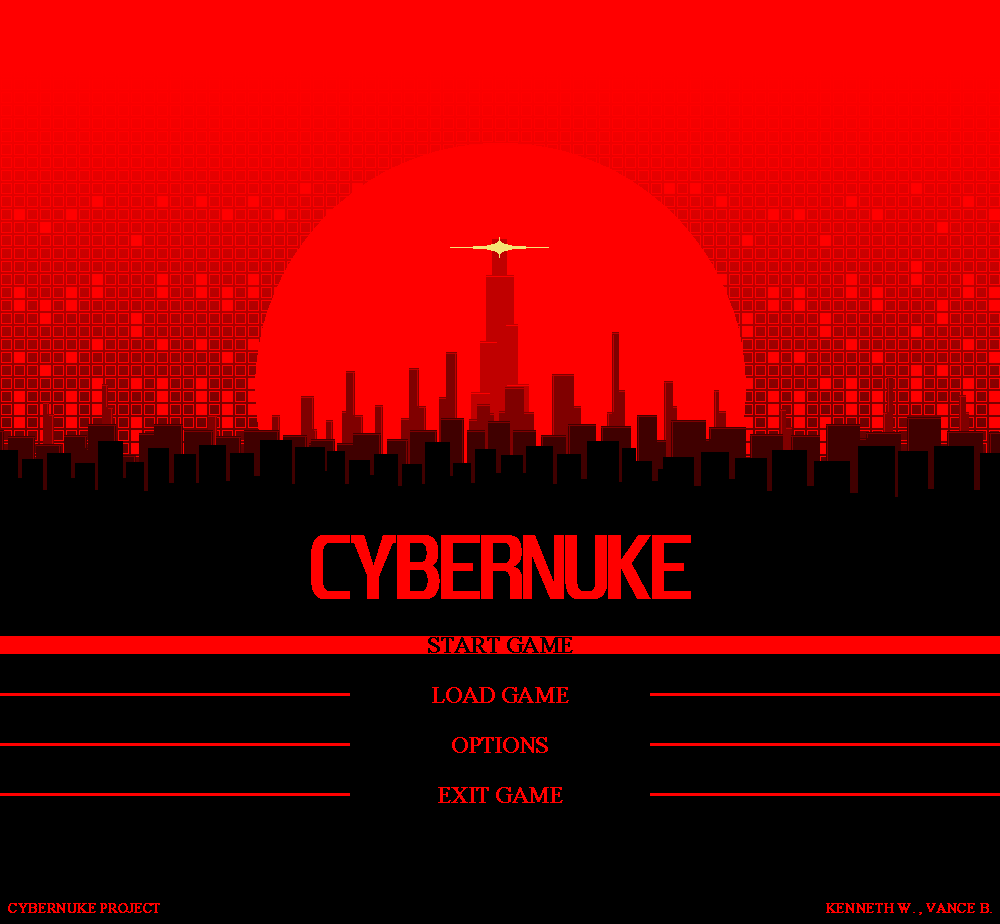
\includegraphics[height=462px, width=500px]{Mockups/CYBERNUKE_MAIN_MENU_2.png}
\caption{CYBERNUKE Main Menu Screen Mockup. Where “Start Game” would start a new game for the player, “Load Game” would allow the player to load a previously saved game, “Options” would allow the player to change options like screen resolution and volume, and “Exit Game” would let the player exit the game.}
\label{main_menu_mockup}
\end{figure}

%Summon Page Break
\pagebreak
The following is a mock-up of CYBERNUKE's combat screen.
\begin{figure}[ht!]
\centering
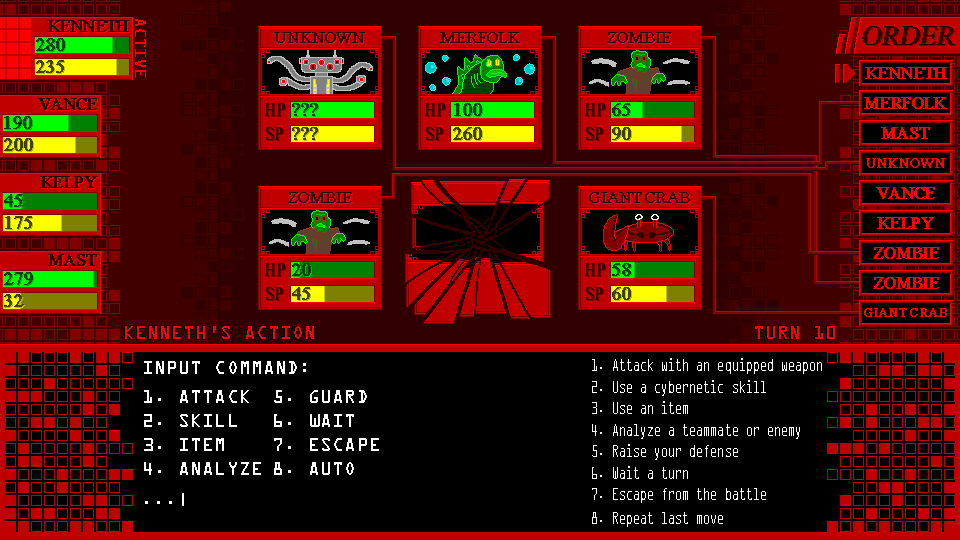
\includegraphics[height=281.25px, width=500px]{Mockups/CYBERNUKE_COMBAT_MOCKUP.png}
\caption{CYBERNUKE Combat Screen Mockup. Where “Attack” lets the player attack an enemy, “Skill” lets the player use a skill, “Item” lets the player use an item from the inventory, “Analyze” lets the player view the stats of a friendly or enemy, “Guard” lets the player raise their defense and end their turn, “Wait” lets the player skip their turn, “Escape” lets the player flee the battle, and “Auto” repeats the character's last action.}
\label{combat_mockup}
\end{figure}


%Ultimate Page Break Attack
\pagebreak
% PROJECT TIMELINE ********************************************************************* %
\section{Project Timeline}

\underline{1. Requirements}
\vspace{5px}

Feb. 4 Proposal Draft: The first requirements we identified were based on a set of games we wanted to combine. 

This included features such as:
\begin{enumerate}
\item Operational Interfaces (Main Menu, Option Menu)
\item Maps
\item User Interface (Map Screen, Player HUD)
\item Character Movement, Interaction
\item Character Interface (Name, Stats)
\item Enemies, Enemy Encounters
\item Combat, Combat Interface
\item Player Saves \& Load Menu
\end{enumerate}

Along with stretch-goals such as:
\begin{enumerate}
\item Companions and Party System
\item Hacking Puzzles
\item More Enemy Types
\item More Story Content
\item Items, Loot, Weapons, Armor, etc.
\item Cybernetic Augmentation
\item Leveling System
\item Currency and Merchants
\item Expanded Character Creation (Species, Backstory, etc.)\\
\end{enumerate}

Feb. 28 Proposal Update: 
No changes in requirements from the proposed draft.\\

Apr. 10 Project Update: 
Implementation was started and we changed the requirements to better the fit MVVM design pattern we had adopted for CYBERNUKE.

Updated requirements:
\begin{enumerate}
\item Operational Interfaces (Main Menu, Combat Menu, Town Menu, etc.)
\item Menu-switching Functionality
\item Secondary Interfaces (Character Menu, Inventory Menu)
\item Enemies
\item Overworld Maps and Map Rendering
\item Overworld Map Functionality (Character Movement, Interaction, Enemy Encounters)
\item Combat Implementation
\item Player Saves \& Load Menu
\end{enumerate}

The stretch-goals were not updated.\\

Apr. 21 Penultimate Update: 
Due to time constraints we removed unnecessary features and made them stretch-goals.

Updated requirements:
\begin{enumerate}
\item Operational Interfaces (Main Menu, Combat Menu, Town Menu, Overworld Menu, Cutscene Menu)
\item Menu Switching
\item Secondary Interfaces (Pause Menu)
\item Enemies \& Enemy Party \& Enemy Data Files
\item Overworld Maps
\item Character-Map Interaction
\item Enemy Encounters
\item Combat
\item Companions and Party System
\item Basic Item System
\end{enumerate}

Updated stretch-goals:
\begin{enumerate}
\item Items, Loot, Weapons, Armor
\item Currency and Merchants
\item Leveling System
\item More Enemy Types
\item Saving and Loading
\item Hacking Puzzles
\item Story Content\\
\end{enumerate}

Apr. 28 Final Presentation: 
Requirements were not changed from the last update.

\vspace{5px}
\underline{2. Design}
\vspace{5px}

Feb. 4 Proposal Draft: Design drafts were made on paper.\\

Feb. 28 Proposal Update: UML design was started.\\

Apr. 10 Project Update: UML was re-factored for the new MVVM design pattern being used.\\

Apr. 21 Penultimate Update: UML was worked on to accomodate new implementations.\\

Apr. 28 Final Presentation: UML was updated to accomodate the new implementations of the Pause Menu, Town Views, User Controls, etc.


This stage resulted in the creation of the first UML diagram for CYBERNUKE.

\vspace{5px}
\underline{3. Implementation}
\vspace{5px}

Feb. 4 Proposal Draft: No implementation done.\\

Feb. 28 Proposal Update: No implementation done.\\

Apr. 10 Project Update: By this point we had the main menu 90\% done, it was missing functionality that let it switch between windows on its own. The combat menu was bare-bones and non-functional. The town, overworld, and cutscene menus were un-implemented but their framework was ready.\\

Apr. 21 Penultimate Update: The combat menu, overworld menu, and town menu were being worked on with the overworld menu being the closest to finished.\\

Apr. 28 Final Presentation: The pause menu, town menu, overworld menu, cutscene menu , and combat menu were fully implemented and the game was finished.

\vspace{5px}
\underline{4. Testing}
\vspace{5px}

Feb. 4 Proposal Draft: No testing done.\\

Feb. 28 Proposal Update: No testing done.\\

Apr. 10 Project Update: Main menu functionality was verified.\\

Apr. 21 Penultimate Update: Overworld functionality was verified. Testing began on combat and town menus.\\

Apr. 28 Final Presentation: Functionality of all menus was verified before the presentation.

\vspace{5px}
\underline{5. Maintenance}
\vspace{5px}

OMITTED.


% PROJECT STRUCTURE ******************************************************************** %
\section{Project Structure}

The basis of Cybernuke's structure is built on top of the MVVM (Model-View-ViewModel) pattern, a variant of the Observer design pattern. MVVM allows us to build Windows, referred to as “Views”, that contain the functionality of a menu. For instance, the MainMenuView is graphically the main menu of the game, and the CombatView is graphically the GUI and functions used in facilitating combat between the player and enemies. The main code and functionality for the views is located in each view's xaml.cs file. Each View will have functionality that allows said view to navigate to other views: for example, the CombatView will be able to navigate to the OverworldView, and vice versa upon finishing and starting combat.

\begin{itemize}

\item The MainMenuView, (which is opened as the initial menu available to the player upon launching the game) it connects to the CutsceneView and OverworldView when starting the game.

\item The CombatView is connected to the OverworldView which randomly decides enemy encounters using a randomized percent-based system where each step you take has a random chance to start an enemy encounter depending on the values set in the map's file. Inside the CombatView, data is pulled from the MainWindow which stores all of the persistent data such as character information, what map you're on, etc. It then stores that information locally within the CombatView and uses it throughout the battle.

\item For the OverworldView, this will serve as the player's method for moving throughout the game's world and exploring locations and places of interest. This is done through use of a grid-like movement system where the player can move one tile each action to cover distance. During each movement step, chances of a random encounter will be factored depending on the location the player is in (for instance, the player will not have random encounters in a safe-designated area while having lots of encounters in "dungeons").

\item From the OverworldView, the player can open the Pause Menu, which functions to allow the player to examine character info, and the more general map (of the current map's layout), as well as closing the Pause Menu and exiting the game.

\item For the TownView (accessed upon reaching a town in the OverworldView), the user will use a sequence of buttons to access features the town holds. For example, to visit certain NPCs, clickable buttons will be used to do that. To visit shops and leave the town, buttons will be used for that as well. The ability to save and load game is available here as well.

\item Finally, the CutsceneView relies on data files to display images and text dialogue.

\end{itemize}

\subsection{UML Outline}

\subsection{Design Patterns Used}
\underline{1. Decorator Design Pattern}
\vspace{5px}

We used a Decorator for the Pause Menu in CYBERNUKE. When opening the Pause Menu it unhides a Content Presenter that is present on the MainWindow. This Content Presenter holds the Pause Menu and renders over the underlying window so that the user cannot accidentally activate anything while paused.

In the UML, the Pause Menu refers to the CharacterView (dubbed as such before becoming known as the Pause Menu). In the constructor for the CharacterView, as stated, it unhides a Content Presenter on the Main Window to prevents the player from taking actions with the Pause Menu open.

\underline{2. MVVM (Model-View-ViewModel) Design Pattern}
\vspace{5px}

We used the MVVM design pattern for CYBERNUKE. We chose to use it as it would allow the program to seamlessly switch between menus without breaking the user's immersion in the game. It also allows us to store data in MainWindow as it stays open persistently.

This is seen very clearly in the UML as the sections are split mainly into the MVVM manager, the different Views used in CYBERNUKE's coding, as well as the Models and ViewModels associated with them.


% RESULTS ****************************************************************************** %
\section{Results}
With the amount of time and experience we had starting off, we were able to get a lot implemented successfully:
\begin{itemize}
\item Operational interfaces. We were able to get a functioning main menu, combat menu, overworld menu, and town menu all working.
\item Menu switching. We were able to implement buttons that allowed players to switch between the different in-game menus.
\item Pause Menu. We got the pause menu working, only in the overworld menu though.
\item Map Files. Maps are loaded in from .txt files stored in the game's files.
\item Enemies, Enemy parties, and Enemy data. We were able to get enemies to load in from files and then load them into combat through enemy party files.
\item Enemy Encounters in the overworld. We were able to implement enemy encounters when in the overworld through the map's data file.
\item Combat menu. We got the combat menu to work where players and enemies can attack each other.
\item Companion and party system. We got the game to load in multiple player characters in the overworld and combat menu.
\item Basic item system. We got a basic item system with armor and weapons able to be equipped by players.
\end{itemize}

We over-estimated the amount of work we would be able to complete in the time we had. This led to a lot of planned features being scrapped and moved to the “Stretch-goals” section of the scope.
A list of features we had to remove:
\begin{itemize}
\item Player and Enemy physical and elemental resistances. This feature required too much in terms of programming and our code wasn't able to handle it.
\item Music and Sounds. Our lack of knowledge in threading led to this being scrapped after numerous attempts at implementing it.
\item Fleshed out armor and weapon system. We originally had slots for 3 armor pieces and a melee + ranged weapon. This had to be cut down to a single Armor and Weapon slot in each character's inventory.
\item Inventory system. This would've included multiple different item types such as consumbles, armors, weapons, quest items, etc. It had to be scrapped due to time constraints.
\item Save/Load system. While possible, we were limited by the amount of time we had which prevented implementation.
\item Game story. We weren't able to get all fundamental features down so a Story was out of question with the time we had left.
\item Merchants and currency. Time constraints.
\item Hacking puzzles. Time constraints.
\item More enemy types. Time constraints.
\end{itemize}

\subsection{Future Work}
We learned a lot about UMLs, WPF, C\#, and game design while working on CYBERNUKE. Although we will continue working on games it won't be on CYBERNUKE and most certainly won't be on WPF. If anything it will end up on our resumes and that will be the end of it.


% BIBLIOGRAPHY ************************************************************************* %
\bibliographystyle{IEEEtran}
\bibliography{./reference}

\begin{thebibliography}{1}

\bibitem{IEEEhowto:cyberpunk}
Britannica, T. Editors of Encyclopaedia. \emph{"cyberpunk."} Encyclopedia Britannica, 1999. https://www.britannica.com/art/cyberpunk.

\bibitem{IEEEhowto:roguelite_1}
Wiktionary. \emph{"roguelite"}
https://en.wiktionary.org/wiki/rogue-lite

\bibitem{IEEEhowto:roguelite_2}
whatNerd, Joel Lee. \emph{"What’s a Roguelike vs. Roguelite? Is the Difference Really That Important?"} whatNerd, 2021. https://whatnerd.com/what-is-a-roguelike-roguelite-difference/.

\end{thebibliography}

% END ********************************************************************************** %
\end{document}
